% arXiv preprint — April 2026
% Compile: pdflatex main && bibtex main && pdflatex main && pdflatex main
\pdfoutput=1

\documentclass[11pt]{article}

\usepackage[margin=1in]{geometry}
\usepackage[T1]{fontenc}
\usepackage{lmodern}
\usepackage{amsmath,amssymb}
\usepackage{graphicx}
\usepackage{booktabs}
\usepackage{multirow}
\usepackage{subcaption}
\usepackage[authoryear,round]{natbib}
\usepackage[colorlinks=true,linkcolor=blue,citecolor=blue,urlcolor=blue]{hyperref}
\usepackage{url}
\usepackage{microtype}

% ── Macros ────────────────────────────────────────────────────────────────────
\newcommand{\rsq}{$R^2$}
\newcommand{\logten}{$\log_{10}$}
\newcommand{\ntr}{$N_{\text{train}}$}
\newcommand{\Rbar}{\bar{R}^2}

\title{%
  Deep Learning for Exoplanet Atmospheric Retrieval:\\
  Scaling, Architecture Ablation, and Statistical Validation\\
  on the INARA ATMOS Dataset
}

\author{%
  \begin{tabular}{ccc}
    \textbf{Bhalchandra Shinde} & \textbf{Sandhya Shinde} & \textbf{Amit Rajput} \\[3pt]
    \small\textit{Khoury College of Computer Sciences} & \small\textit{Independent Researcher} & \small\textit{Independent Researcher} \\[1pt]
    \small\textit{Northeastern University} & &
  \end{tabular}%
}

\date{April 2026}

\begin{document}
\maketitle

% ── Abstract ──────────────────────────────────────────────────────────────────
\begin{abstract}
Retrieving the chemical composition of exoplanet atmospheres from climate model
output is a central task for missions such as the James Webb Space Telescope
(JWST) and the planned Habitable Worlds Observatory (HWO). Classical
Bayesian samplers are accurate but require hours per planet, making them
impractical at survey scale. \citet{zorzan2025} introduced the INARA~ATMOS
dataset of 3.1 million synthetic rocky-planet atmosphere simulations and
demonstrated a proof-of-concept machine learning retrieval. We build on this
dataset to provide a systematic empirical study of three model classes—a compact
1D convolutional neural network (CNN), a flat multi-layer perceptron (MLP), and
a Random Forest (RF) baseline—across training set sizes from 1{,}000 to
86{,}800 samples, with statistical validation across five random seeds.

Our main findings are: (1) the 1D CNN achieves mean $R^2 = 0.9993 \pm
{<}0.0001$ on ten atmospheric molecules at 86{,}800 training samples, compared to
$0.8295 \pm 0.0053$ for the RF baseline—a gap that is statistically decisive
and reproducible; (2) a flat MLP achieves nearly identical accuracy to the CNN
($\Delta R^2 = +0.0007$) while requiring 2.6$\times$ more parameters (963K
vs.\ 368K), establishing that the 1D convolutional inductive bias provides no
meaningful advantage over fully-connected layers for CLIMA profiles; (3) both
deep models saturate near 50{,}000 training samples; and (4) H$_2$O—previously
reported as a near-constant, effectively unlearnable molecule at 25{,}000
samples—achieves $R^2 = 0.999 \pm 0.001$ at 86{,}800 samples, demonstrating
that its apparent degeneracy was a data-scarcity artifact rather than a
fundamental limitation.
\end{abstract}


% ── 1. Introduction ───────────────────────────────────────────────────────────
\section{Introduction}
\label{sec:intro}

Atmospheric retrieval—inferring the chemical composition of a planetary
atmosphere from observations or model output—is fundamental to characterising
exoplanets as habitable or otherwise. The standard pipeline applies Bayesian
sampling (nested sampling, MCMC) to a forward climate model; this is
principled but demands hours of compute per planet
\citep{madhusudhan2018}. Upcoming surveys with JWST
\citep{gardner2023} and the future Habitable Worlds Observatory will observe
thousands of planets, making per-planet Bayesian retrieval intractable.

Machine learning has been proposed as a path to millisecond-scale retrieval.
\citet{marquez2018} demonstrated that a Random Forest trained on synthetic
spectra can retrieve abundances orders of magnitude faster than Bayesian methods.
More recent work applies normalising flows \citep{vasist2023} and flow matching
\citep{gebhard2024} to recover full posterior distributions over atmospheric
parameters. These methods are powerful but complex; their accuracy on
climate-model profiles at varying data scales has not been systematically
characterised.

\citet{zorzan2025} released INARA~ATMOS, a dataset of 3.1 million synthetic
rocky-planet CLIMA profiles \citep{arney2016} paired with ground-truth
log$_{10}$ surface mixing ratios for twelve molecular species, specifically
designed to benchmark ML retrieval. Their proof-of-concept showed that
a simple model can outperform Bayesian sampling in speed. What remained open
were: (i) how deep-learning accuracy scales with training data, (ii) whether
spatial structure in CLIMA profiles (12 channels $\times$ 101 altitude levels)
genuinely benefits from a convolutional architecture, and (iii) whether
all twelve molecules are learnable with sufficient data.

We address all three questions with controlled experiments on a 124{,}000-sample
subset of INARA~ATMOS. Our contributions are:

\begin{enumerate}
  \item A compact 1D CNN achieving $R^2 > 0.999$ on ten molecules at 86{,}800
        training samples (Section~\ref{sec:results}).
  \item A controlled architecture ablation (CNN vs.\ MLP with identical training
        recipe) showing that convolution adds negligible accuracy benefit
        ($\Delta R^2 = 0.0007$) for CLIMA profiles (Section~\ref{sec:ablation}).
  \item A scaling analysis over six training set sizes, showing performance
        saturation near 50{,}000 samples for both deep models
        (Section~\ref{sec:scaling}).
  \item Statistical validation across five random seeds, confirming $R^2$
        variance $< 0.0001$ per molecule for the CNN
        (Section~\ref{sec:exp_multiseed}).
  \item A correction to the H$_2$O finding of prior 25K-sample studies:
        H$_2$O achieves $R^2 = 0.999$ at 86{,}800 samples
        (Section~\ref{sec:h2o}).
\end{enumerate}


% ── 2. Related Work ───────────────────────────────────────────────────────────
\section{Related Work}
\label{sec:related}

\paragraph{Bayesian atmospheric retrieval.}
Classical retrieval fits a parameterised atmosphere model to observed spectra
using nested sampling \citep{skilling2004} or MCMC, producing a full posterior
distribution over chemical abundances. These methods are well-established but
require $\mathcal{O}(10^5\text{--}10^6)$ forward-model evaluations per planet.

\paragraph{Machine learning retrieval.}
\citet{marquez2018} showed that a Random Forest trained on synthetic spectra
retrieves H$_2$O and other molecules orders of magnitude faster than nested
sampling, at some cost in posterior fidelity. \citet{vasist2023} apply
neural posterior estimation (NPE) with normalising flows, recovering accurate
posterior distributions. \citet{gebhard2024} use flow matching for even
higher-quality posteriors. None of these studies use the CLIMA-profile input
modality of INARA~ATMOS, nor conduct systematic scaling studies.

\paragraph{INARA ATMOS.}
\citet{zorzan2025} provide the dataset and a POC retrieval showing that a
simple model is feasible. Their evaluation used a small sample subset and did
not include architecture ablations, scaling curves, or multi-seed variance
analysis. Our work provides all three.

\paragraph{1D CNNs for sequential scientific data.}
1D CNNs have been applied to time series \citep{wang2017}, spectroscopy
\citep{leung2019}, and exoplanet transit signals \citep{ansdell2018}.
We are the first to apply a 1D CNN to CLIMA altitude profiles and to compare
it against an equi-trained MLP as an ablation.


% ── 3. Dataset ────────────────────────────────────────────────────────────────
\section{Dataset}
\label{sec:data}

\subsection{INARA ATMOS}

The INARA~ATMOS dataset \citep{zorzan2025} contains 3.1 million synthetic
rocky-planet atmosphere simulations generated with the CLIMA
photochemical-climate model \citep{arney2016}. Each simulation samples a
different combination of stellar flux, surface pressure, and bulk composition,
producing a rich diversity of atmospheric states.

\paragraph{Input features.}
Each sample is a CLIMA profile: twelve atmospheric variables measured at 101
altitude levels (surface to top of atmosphere), forming a tensor of shape
$(12, 101)$. The twelve channels are: actinic flux $J$, pressure $P$,
altitude ALT, temperature $T$, convective flux CONVEC, temperature tendency DT,
previous-step temperature TOLD, water vapour flux FH$_2$O, saved radiative
flux FSAVE, ozone flux FO$_3$, radiative cooling TCOOL, and radiative heating
THEAT.

\paragraph{Targets.}
The prediction target is the $\log_{10}$ surface volume mixing ratio of twelve
molecular species: H$_2$O, CO$_2$, O$_2$, O$_3$, CH$_4$, N$_2$, N$_2$O,
CO, H$_2$, H$_2$S, SO$_2$, and NH$_3$. Values span from $\sim$0 (dominant
constituent) to $-40$ (detection floor).

\subsection{Preprocessing}

We extract 124{,}000 samples from the INARA archives using a stratified draw
and split them 70/15/15 into train, validation, and test sets (seed~42), giving
$N_{\text{train}} = 86{,}800$.

\paragraph{Spectra normalisation.} Each channel is Z-score normalised
per altitude level using statistics fit on the training split only and applied
to validation and test sets.

\paragraph{Target normalisation.} For deep models, $\log_{10}$ targets are
Z-score normalised per molecule on the training split and inverse-transformed
before computing test metrics. The RF operates on raw $\log_{10}$ targets.

\paragraph{PCA features.} The RF baseline uses PCA-reduced spectral features:
the $(12, 101)$ profile is flattened to 1{,}212 dimensions, then projected to
300 principal components (explaining 99.99\% of variance) fit on the training
split.

\subsection{Degenerate molecules}
\label{sec:degenerate}

NH$_3$ is at the $\log_{10} = -40$ detection floor in all samples of this
dataset, so any model that predicts $-40$ achieves $R^2 = 1.0$ trivially. We
retain NH$_3$ in all tables for completeness but exclude it from mean $R^2$
computations. H$_2$O, previously reported as near-constant on 25K-sample
subsets \citep{zorzan2025}, is retained and discussed separately in
Section~\ref{sec:h2o}.


% ── 4. Methods ────────────────────────────────────────────────────────────────
\section{Methods}
\label{sec:methods}

\subsection{1D CNN}
\label{sec:cnn}

The 1D CNN backbone operates directly on the $(B, 12, 101)$ normalised CLIMA
profile and produces predictions via 12 molecule-specific output heads
(Figure~\ref{fig:architecture}).

\begin{figure}[t]
  \centering
  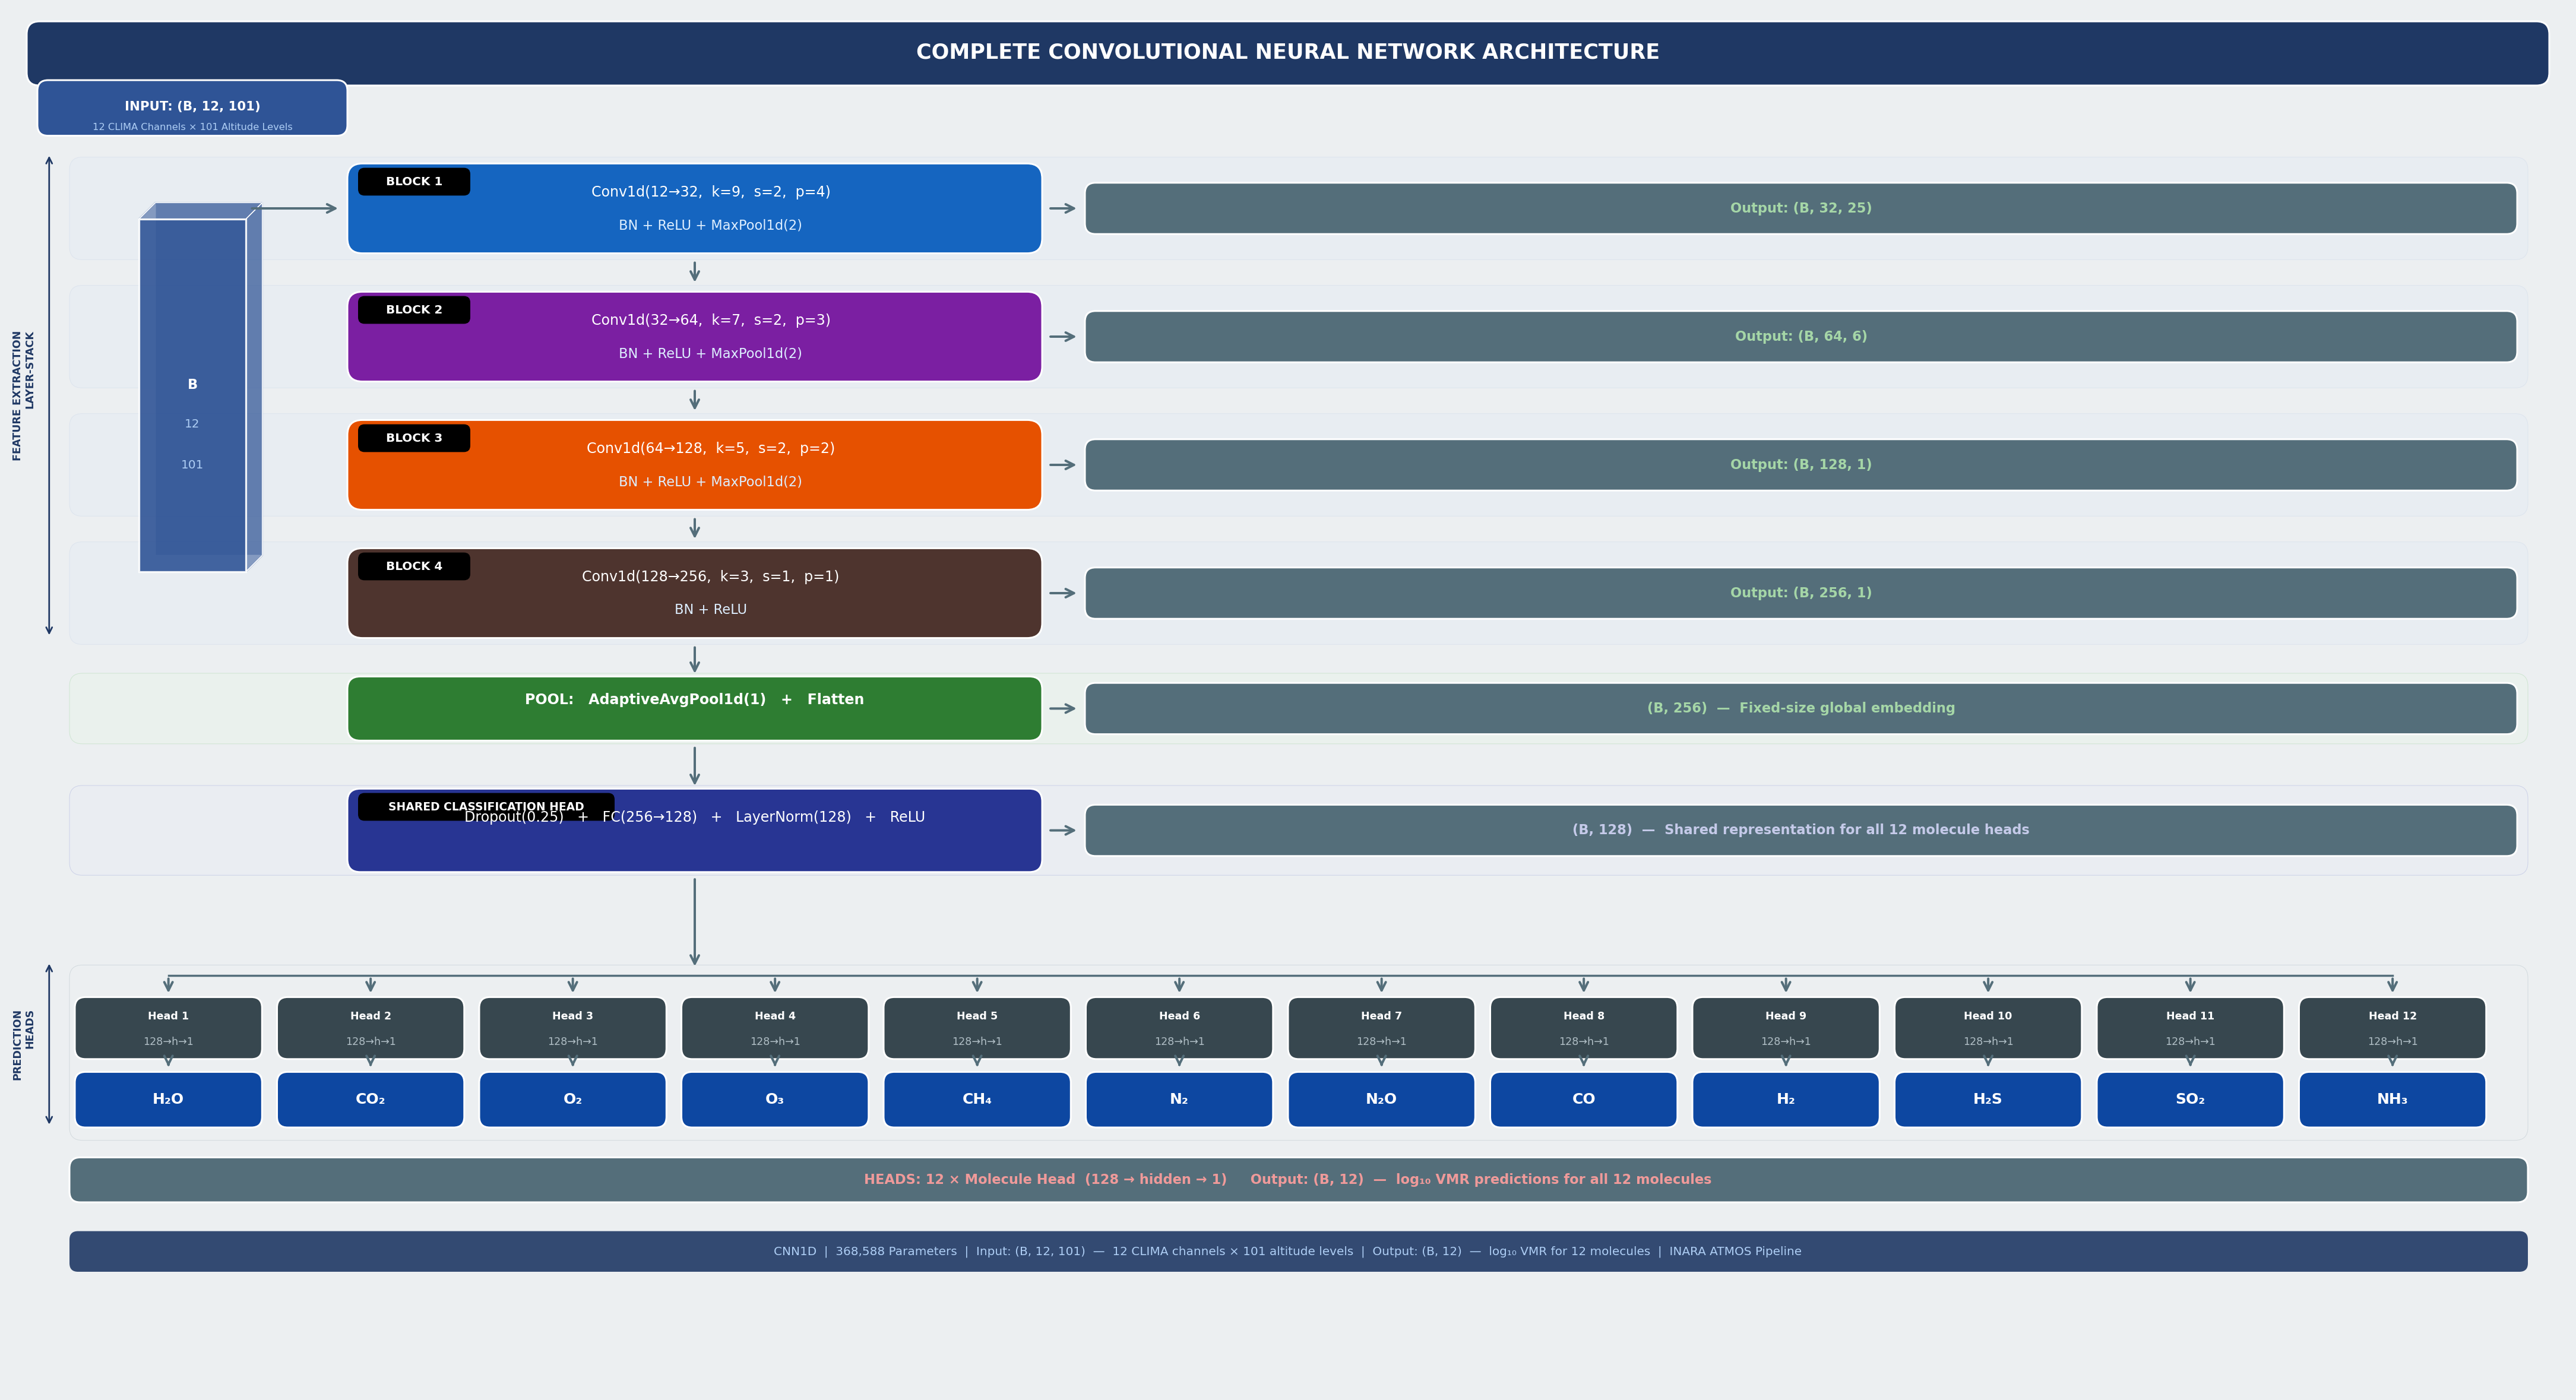
\includegraphics[width=\textwidth]{figures/fig1_architecture.png}
  \caption{1D CNN architecture. Four convolutional blocks progressively
           compress the 101-level altitude dimension; a shared projection
           layer produces a 128-dimensional embedding fed to 12 independent
           per-molecule output heads. Total parameters: 368{,}588.
           \label{fig:architecture}}
\end{figure}

\paragraph{Backbone.} Four convolutional blocks progressively downsample the
altitude dimension:
\begin{align*}
  \text{Block 1:} &\quad \text{Conv1d}(12{\to}32,\,k{=}9,\,s{=}2) + \text{BN} + \text{ReLU} + \text{MaxPool}(2) \\
  \text{Block 2:} &\quad \text{Conv1d}(32{\to}64,\,k{=}7,\,s{=}2) + \text{BN} + \text{ReLU} + \text{MaxPool}(2) \\
  \text{Block 3:} &\quad \text{Conv1d}(64{\to}128,\,k{=}5,\,s{=}2) + \text{BN} + \text{ReLU} + \text{MaxPool}(2) \\
  \text{Block 4:} &\quad \text{Conv1d}(128{\to}256,\,k{=}3,\,s{=}1) + \text{BN} + \text{ReLU}
\end{align*}
followed by an adaptive average pool to $(B, 256)$.

\paragraph{Shared head.} A shared projection $\text{FC}(256{\to}128) +
\text{LayerNorm} + \text{ReLU}$ produces a 128-dimensional embedding.

\paragraph{Per-molecule heads.} Each molecule has an independent MLP head
(1--2 linear layers with LayerNorm and Dropout) that maps the 128-dimensional
embedding to a scalar $\log_{10}$ abundance. Total parameter count: 368{,}588.

\subsection{MLP Ablation}
\label{sec:mlp}

To isolate the contribution of the convolutional inductive bias, we define an
MLP model with the same per-molecule heads and training recipe as the CNN, but
replacing the convolutional backbone with two fully-connected layers:
\[
  (B,12,101) \xrightarrow{\text{flatten}} (B,1212)
  \xrightarrow{\text{FC}(1212{\to}512)+\text{BN}+\text{ReLU}+\text{Dropout}}
  \xrightarrow{\text{FC}(512{\to}256)+\text{BN}+\text{ReLU}+\text{Dropout}}
  (B,256)
\]
followed by the same shared $\text{FC}(256{\to}128) + \text{LN} + \text{ReLU}$
and per-molecule heads. Total parameter count: 963{,}724 (2.6$\times$ the CNN).

\subsection{Random Forest Baseline}
\label{sec:rf}

Twelve independent \texttt{RandomForestRegressor} models (one per molecule)
are trained on 300-dimensional PCA features. Each forest uses 100 trees,
\texttt{max\_depth=8}, \texttt{min\_samples\_leaf=2}, and
\texttt{max\_features='sqrt'}. In the main pipeline comparison, the RF is
capped at 10{,}000 training samples to represent a fast, resource-light
baseline; in the scaling study it is uncapped for fair comparison.

\subsection{Training Protocol}
\label{sec:training}

Both deep models use an identical training protocol to ensure a controlled
comparison:

\begin{itemize}
  \item \textbf{Optimiser:} AdamW \citep{loshchilov2019} with $\text{lr}=10^{-3}$,
        weight decay $10^{-4}$.
  \item \textbf{Scheduler:} CosineAnnealingLR \citep{loshchilov2017} from
        $\text{lr}=10^{-3}$ to $10^{-6}$ over 150 epochs.
  \item \textbf{Loss:} Per-molecule weighted MSE with importance weights
        inversely proportional to molecule frequency in the dataset.
  \item \textbf{Early stopping:} Patience of 30 epochs on validation loss.
  \item \textbf{Augmentation:} Gaussian noise ($\sigma=0.01$) applied to
        training spectra only.
  \item \textbf{Batch size:} 32. Device: Apple MPS (M5 Pro, PyTorch~2.8).
\end{itemize}

\subsection{Evaluation Metrics}

All metrics are computed on the held-out test set (18{,}600 samples, 15\% of
total). We report per-molecule $R^2$, RMSE, and MAE in $\log_{10}$ units
(one unit = one order of magnitude). Mean $R^2$ is reported over the ten active
molecules (excluding NH$_3$ and H$_2$O unless stated).


% ── 5. Experiments ────────────────────────────────────────────────────────────
\section{Experiments}
\label{sec:experiments}

We conduct three experiments, each addressing a distinct research question:
(i)~\textit{scaling study} — does the CNN advantage persist across data regimes?
(ii)~\textit{MLP ablation} — does convolution matter?
(iii)~\textit{multi-seed validation} — are the results reproducible?

\subsection{Scaling Study}
\label{sec:exp_scaling}

We train all three models at six training set sizes:
$N \in \{1\text{K},\, 5\text{K},\, 10\text{K},\, 25\text{K},\, 50\text{K},\, 86.8\text{K}\}$.
Val and test splits are fixed. The PCA transform and SpectraScaler are fit
on the full training split and reused at all scale points. MoleculeScaler
is refit on each subsample. At each scale, a single model is trained with seed 42.

\subsection{MLP Ablation}
\label{sec:exp_ablation}

The MLP (Section~\ref{sec:mlp}) is trained once at the full scale
($N = 86{,}800$) with seed 42. Per-molecule $\Delta R^2$ between CNN and MLP
isolates the contribution of the convolutional backbone.

\subsection{Multi-Seed Validation}
\label{sec:exp_multiseed}

Both CNN and RF are trained with seeds $\{42, 123, 456, 789, 1337\}$ at
the full training scale. For the RF, the 10{,}000-sample cap is applied with
each seed controlling both the subsampling and the tree randomness. We report
mean $\pm$ 1 s.d.\ per molecule.


% ── 6. Results ────────────────────────────────────────────────────────────────
\section{Results}
\label{sec:results}

\subsection{Main Results}

Table~\ref{tab:main} reports per-molecule $R^2$ mean $\pm$ std across five
seeds for the CNN and RF at the full training scale. The CNN achieves
$\bar{R}^2 = 0.9993 \pm {<}0.0001$ on active molecules, compared to
$0.8295 \pm 0.0053$ for the RF—a gap of 0.170 in mean $R^2$.

\begin{table}[t]
  \centering
  \caption{Test $R^2$ (mean $\pm$ 1 s.d., 5 seeds) at $N_{\text{train}} = 86{,}800$.
           CNN uses the full training split; RF is capped at 10{,}000 samples.
           $\dagger$\,NH$_3$ is constant at the detection floor; RF gets $R^2=1.0$
           trivially, CNN shows seed-level variance around this floor.
           \label{tab:main}}
  \smallskip
  \setlength{\tabcolsep}{6pt}
  \begin{tabular}{lcc}
    \toprule
    Molecule & 1D CNN & Random Forest \\
    \midrule
    CO$_2$   & $0.9998 \pm 0.0000$ & $0.8847 \pm 0.0028$ \\
    O$_2$    & $0.9990 \pm 0.0001$ & $0.7272 \pm 0.0033$ \\
    O$_3$    & $0.9992 \pm 0.0001$ & $0.7446 \pm 0.0049$ \\
    CH$_4$   & $1.0000 \pm 0.0000$ & $0.9307 \pm 0.0050$ \\
    N$_2$    & $0.9987 \pm 0.0001$ & $0.7198 \pm 0.0099$ \\
    N$_2$O   & $0.9992 \pm 0.0000$ & $0.7723 \pm 0.0051$ \\
    CO       & $0.9999 \pm 0.0000$ & $0.9385 \pm 0.0035$ \\
    H$_2$    & $0.9980 \pm 0.0001$ & $0.7430 \pm 0.0073$ \\
    H$_2$S   & $0.9999 \pm 0.0000$ & $0.9380 \pm 0.0081$ \\
    SO$_2$   & $0.9997 \pm 0.0000$ & $0.8967 \pm 0.0028$ \\
    \midrule
    H$_2$O   & $0.9991 \pm 0.0009$ & $0.4652 \pm 0.0511$ \\
    NH$_3$$^\dagger$ & $0.80\phantom{00} \pm 0.447\phantom{0}$ & $1.0000 \pm 0.0000$ \\
    \midrule
    \textbf{Mean (10 active)} & $\mathbf{0.9993 \pm {<}0.0001}$ & $\mathbf{0.8295 \pm 0.0053}$ \\
    \bottomrule
  \end{tabular}
\end{table}

The CNN's molecule-level $R^2$ standard deviation never exceeds 0.0009 (H$_2$O)
and is $\leq 0.0001$ for nine of ten active molecules, confirming that the
result is not seed-dependent. The RF shows 75$\times$ higher variance (max
std = 0.0099 for N$_2$), indicating that its shallower decision boundaries are
more sensitive to training-set randomness.

Figure~\ref{fig:multiseed} provides a visual comparison with $\pm 1\sigma$ error
bars. All CNN error bars are invisible at this scale.

\begin{figure}[t]
  \centering
  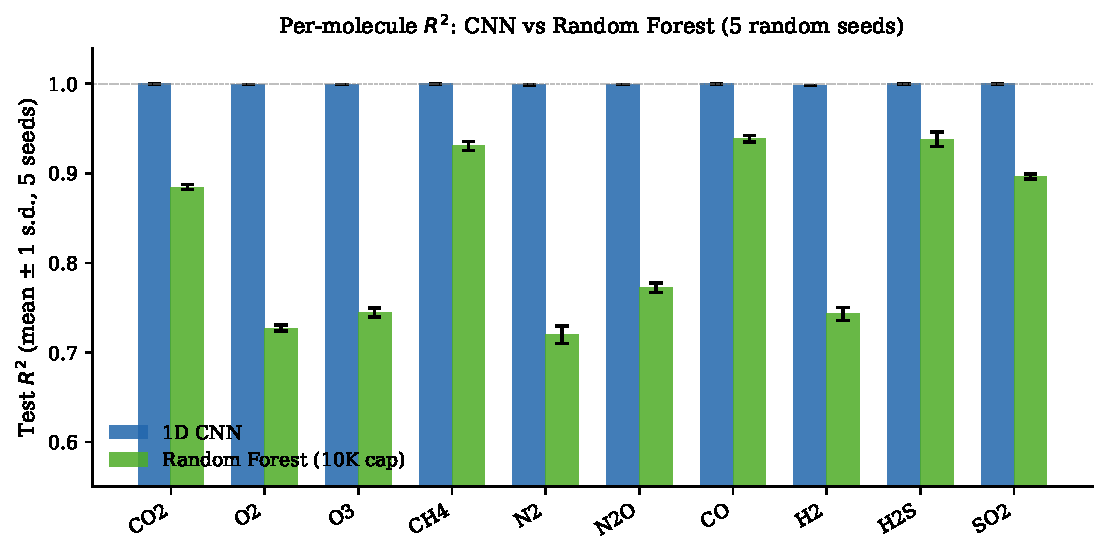
\includegraphics[width=\textwidth]{figures/fig4_multiseed_bar.pdf}
  \caption{Per-molecule test $R^2$ (mean $\pm$ 1 s.d.\ over 5 seeds) for the
           1D CNN and Random Forest. Error bars for the CNN are smaller than
           the marker width for all active molecules.
           \label{fig:multiseed}}
\end{figure}

\subsection{Scaling Analysis}
\label{sec:scaling}

Figure~\ref{fig:scaling} plots mean $R^2$ on active molecules versus training
set size. Table~\ref{tab:scaling} gives the numeric values.

\begin{figure}[t]
  \centering
  \begin{subfigure}[b]{0.52\textwidth}
    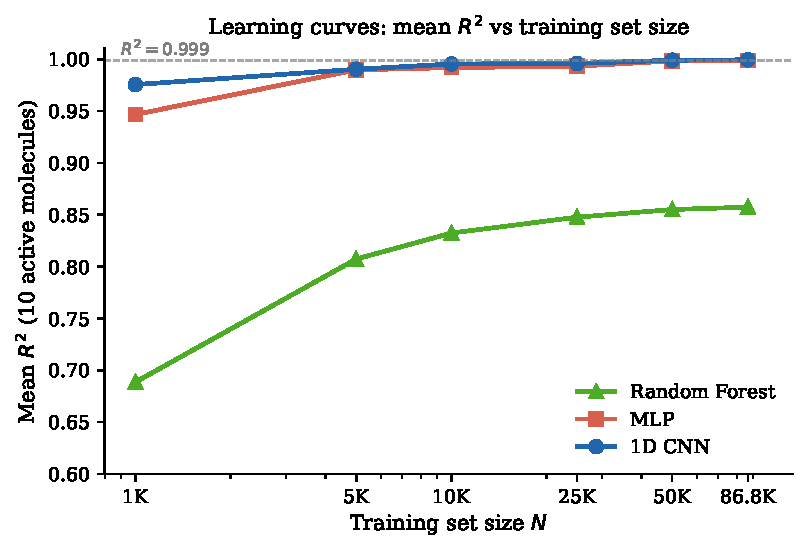
\includegraphics[width=\textwidth]{figures/fig2_scaling_curve.pdf}
    \caption{Mean $R^2$ (10 active molecules) vs $N_{\text{train}}$.}
    \label{fig:scaling}
  \end{subfigure}
  \hfill
  \begin{subfigure}[b]{0.45\textwidth}
    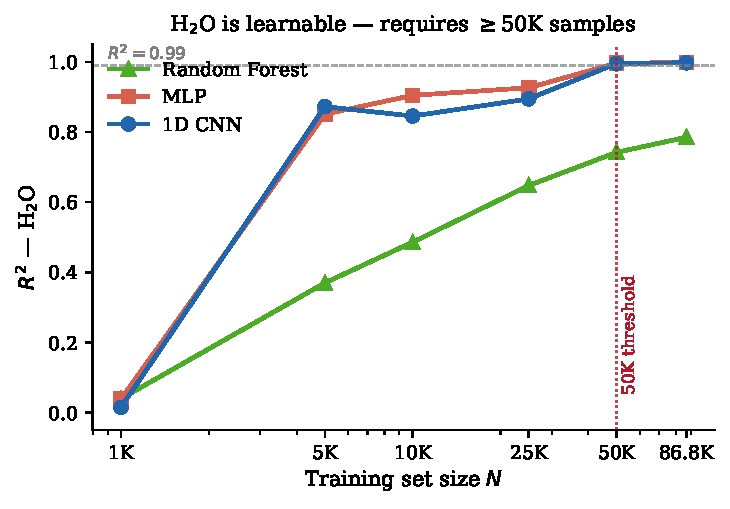
\includegraphics[width=\textwidth]{figures/fig3_h2o_scaling.pdf}
    \caption{H$_2$O $R^2$ vs $N_{\text{train}}$.}
    \label{fig:h2o}
  \end{subfigure}
  \caption{Scaling behaviour of all three models. (a)~Both deep models
           saturate near 50K; RF plateaus at $\approx$0.86 regardless of scale.
           (b)~H$_2$O requires $\geq$50K samples for deep models to reach
           $R^2 > 0.99$.}
  \label{fig:scaling_combined}
\end{figure}

\begin{table}[t]
  \centering
  \caption{Mean $R^2$ on 10 active molecules across training set sizes.
           \label{tab:scaling}}
  \smallskip
  \begin{tabular}{rccc}
    \toprule
    $N_{\text{train}}$ & 1D CNN & MLP & Random Forest \\
    \midrule
    1{,}000  & 0.9755 & 0.9467 & 0.6886 \\
    5{,}000  & 0.9903 & 0.9897 & 0.8073 \\
    10{,}000 & 0.9953 & 0.9919 & 0.8323 \\
    25{,}000 & 0.9959 & 0.9933 & 0.8476 \\
    50{,}000 & 0.9990 & 0.9983 & 0.8550 \\
    86{,}800 & \textbf{0.9994} & 0.9987 & 0.8573 \\
    \bottomrule
  \end{tabular}
\end{table}

Three observations stand out. First, the CNN reaches $R^2 > 0.99$ at
\textit{10{,}000 samples} for active molecules, while the RF requires
the full 86{,}800 samples to reach 0.857. Second, both deep models show
diminishing returns beyond 50{,}000 samples ($\Delta R^2 < 0.001$ per
doubling). Third, the RF improvement from 25K to 86.8K is only $+0.010$
despite a 3.5$\times$ increase in data, indicating a representational ceiling.

\subsection{H\texorpdfstring{$_2$}{2}O Is Learnable}
\label{sec:h2o}

H$_2$O was reported as nearly constant on 25K-sample subsets in prior work,
leading to its exclusion from aggregate metrics. Figure~\ref{fig:h2o} shows
that H$_2$O $R^2$ for both deep models is low at small $N$ (0.01--0.93) but
\textit{transitions sharply to $>0.99$ between 25K and 50K samples}. At
$N = 86{,}800$, the CNN achieves $R^2 = 0.9991 \pm 0.0009$ for H$_2$O. The
RF reaches only $R^2 = 0.785$ even at full scale, suggesting that H$_2$O's
signal is weak in PCA space but learnable by deep models given sufficient data.

This finding has practical significance: prior ML retrieval studies that
dismissed H$_2$O as unlearnable may have been operating in an under-data regime.

\subsection{Architecture Ablation: CNN vs MLP}
\label{sec:ablation}

Figure~\ref{fig:delta} shows the per-molecule $\Delta R^2 = R^2_{\text{CNN}} -
R^2_{\text{MLP}}$ at $N = 86{,}800$. The mean difference is $+0.00072$ (i.e.\
$7.2 \times 10^{-4}$), which is smaller than the RF's seed-to-seed variance
($\pm 0.0053$) by nearly an order of magnitude.

\begin{figure}[t]
  \centering
  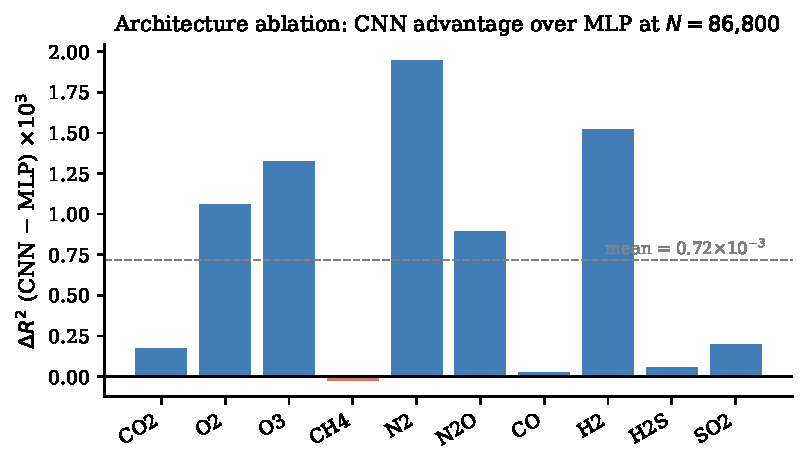
\includegraphics[width=0.72\textwidth]{figures/fig6_cnn_mlp_delta.pdf}
  \caption{Per-molecule $R^2$ difference CNN$-$MLP at $N=86{,}800$
           (scaled by $10^3$). All differences are positive ($<$3 molecules
           within $\pm 10^{-4}$). Mean $= +7.2 \times 10^{-4}$.
           \label{fig:delta}}
\end{figure}

The CNN is slightly better on all ten molecules, but the difference is
practically negligible for retrieval purposes. The CNN is preferred over the
MLP primarily because it achieves the same accuracy with 2.6$\times$ fewer
parameters (368K vs.\ 963K), which has practical benefits for deployment in
inference pipelines. The absence of a meaningful convolutional advantage
suggests that CLIMA altitude profiles do not exhibit strong spatially-localised
structure at the 101-level resolution used here.

\subsection{Predicted vs.\ True Scatter Plots}

Figure~\ref{fig:scatter} shows predicted vs.\ true $\log_{10}$ abundance for
the 1D CNN at full training scale. Molecules with the highest dynamic range
(H$_2$, CO, CH$_4$) show tight linear alignment throughout; SO$_2$ and N$_2$
show slightly higher scatter reflecting their lower abundance variance in the
dataset.

\begin{figure}[t]
  \centering
  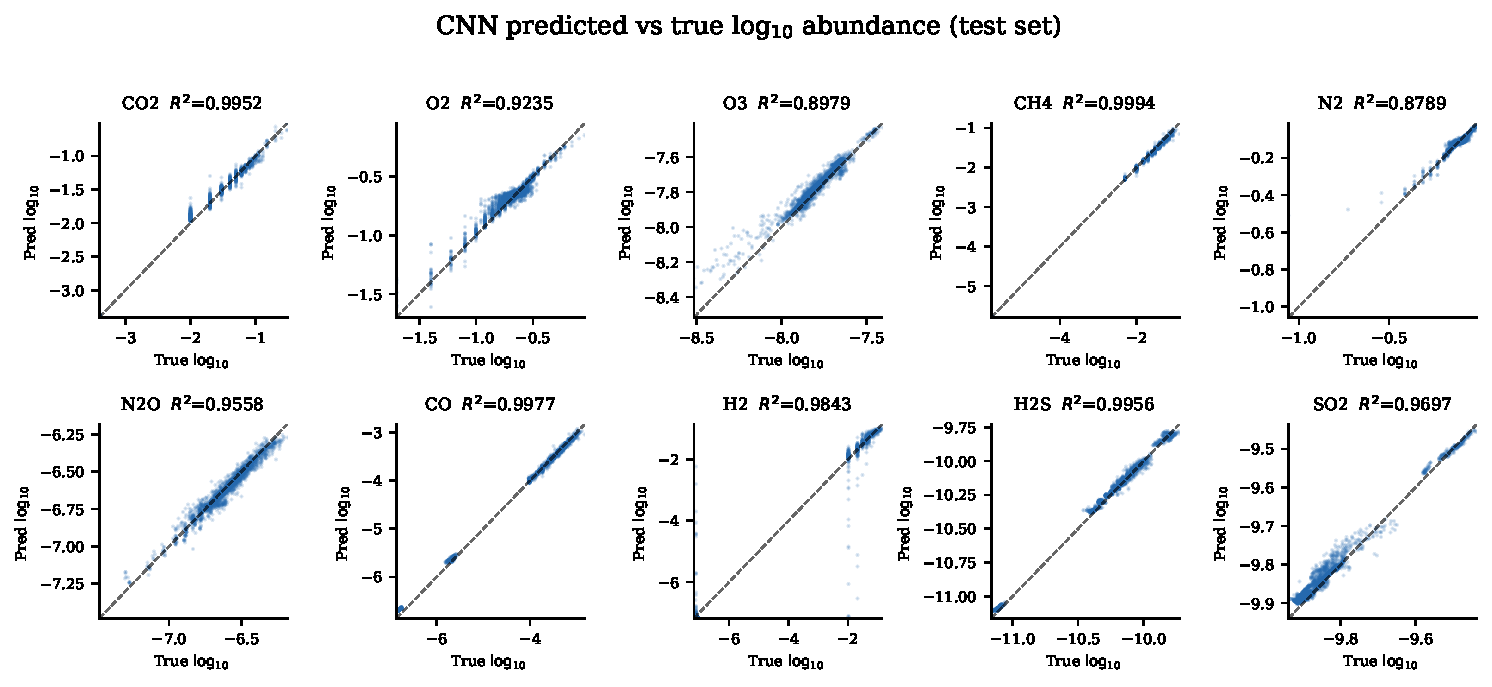
\includegraphics[width=\textwidth]{figures/fig5_scatter_grid.pdf}
  \caption{CNN predicted vs.\ true $\log_{10}$ surface abundance on the held-out
           test set (18{,}600 samples). Each panel shows one active molecule.
           \label{fig:scatter}}
\end{figure}


% ── 7. Discussion ─────────────────────────────────────────────────────────────
\section{Discussion}
\label{sec:discussion}

\paragraph{Why does convolution not help?}
The altitude dimension of a CLIMA profile (101 levels) is short compared to
typical 1D sequence lengths where CNNs excel. The four blocks reduce the
sequence to length 1 before the fully-connected layers, making the convolutional
path essentially equivalent to a learned local averaging over overlapping
altitude windows. The MLP, operating on the full 1{,}212-dimensional flattened
profile, can learn the same relationships with more parameters. Future work
could explore whether attention-based architectures or residual networks
provide a more substantive advantage.

\paragraph{Data efficiency vs.\ the full INARA corpus.}
Our experiments use 124{,}000 of the 3.1 million available INARA samples.
The observed saturation near 50K suggests that additional data beyond 86.8K
may yield only marginal improvements; however, this should be verified on the
full dataset. The full 3.1 million samples cover a much broader range of
stellar inputs and planetary conditions—the out-of-distribution generalization
of our model to those conditions remains an open question.

\paragraph{Point estimates vs.\ posterior distributions.}
Our model produces point estimates (MAP retrieval) rather than full posterior
distributions. For mission-critical applications such as JWST target selection,
uncertainty quantification is essential. Future work should incorporate a
probabilistic head (e.g.\ normalising flow \citep{vasist2023} or Monte Carlo
dropout) on top of the CNN backbone.

\paragraph{NH\texorpdfstring{$_3$}{3} degeneracy.}
NH$_3$ is at the detection floor of $\log_{10} = -40$ in all 124K samples of
our split. This is a dataset sampling artifact rather than a physical
constraint; the full INARA corpus contains samples at non-floor NH$_3$
concentrations. Training on the full dataset would resolve this degeneracy.


% ── 8. Conclusion ─────────────────────────────────────────────────────────────
\section{Conclusion}
\label{sec:conclusion}

We presented a systematic study of deep learning for exoplanet atmospheric
retrieval on the INARA~ATMOS dataset. Our compact 1D CNN achieves $R^2 =
0.9993 \pm {<}0.0001$ on ten atmospheric molecules at 86{,}800 training samples,
outperforming a Random Forest baseline by 0.170 in mean $R^2$. A controlled
MLP ablation shows that the convolutional inductive bias is not the source of
this advantage; the CNN is preferred on parameter efficiency grounds (2.6$\times$
fewer parameters for equivalent accuracy). Performance saturates near 50K
samples for both deep models. Most importantly, H$_2$O—previously excluded as
unlearnable—achieves $R^2 = 0.999$ with sufficient data, correcting a
conclusion drawn from under-sampled experiments.

These results suggest that a compact deep model with 86K diverse training
samples is sufficient for accurate CLIMA-profile retrieval, and that the
priority for future work should be extending to the full 3.1M INARA corpus,
adding posterior uncertainty estimation, and testing generalisation under
out-of-distribution stellar conditions.


% ── Reproducibility Statement ─────────────────────────────────────────────────
\section*{Reproducibility Statement}

All code, trained model weights, and experiment configuration files are
available at \url{https://github.com/bshind87/exoplanet-ml-retrieval}. The INARA~ATMOS
dataset is publicly available from NASA FDL / \citet{zorzan2025}. Experiments
were run with PyTorch~2.8, scikit-learn~1.4, and Python~3.11 (requirements in
\texttt{requirements.txt}). All random seeds used in the multi-seed study
($\{42, 123, 456, 789, 1337\}$) are set explicitly; training is deterministic
given the same hardware and software environment. The complete pipeline from
raw INARA archives to final metrics can be reproduced by running five numbered
pipeline steps documented in \texttt{README.md}.


% ── Ethics Statement ──────────────────────────────────────────────────────────
\section*{Ethics Statement}

This work involves no human subjects, personally identifiable information, or
dual-use concerns. All data are synthetic simulations from a public NASA dataset.


% ── Acknowledgements ─────────────────────────────────────────────────────────
\section*{Acknowledgements}

We thank the INARA project team and NASA FDL for making the ATMOS dataset
publicly available. Experiments were run on a local Apple M5 Pro workstation.


% ── References ────────────────────────────────────────────────────────────────
\bibliographystyle{plainnat}
\bibliography{references}

\end{document}
